%
% Copyright 2018 Joel Feldman, Andrew Rechnitzer and Elyse Yeager.
% This work is licensed under a Creative Commons Attribution-NonCommercial-ShareAlike 4.0 International License.
% https://creativecommons.org/licenses/by-nc-sa/4.0/
%
\questionheader{ex:s1.7}

%%%%%%%%%%%%%%%%%%
\subsection*{\Conceptual}
%%%%%%%%%%%%%%%%%%
\begin{Mquestion}\label{1.7_difftoint}
The method of integration by substitution comes from the $\rule{1.5cm}{0.15mm}$ rule for differentiation.\\
The method of integration by parts comes from the  $\rule{1.5cm}{0.15mm}$ rule for differentiation.
\end{Mquestion}
\begin{hint}
Read back over Sections~\eref{CLP101}{sec subs} and \eref{CLP101}{sec intbyparts}
of the CLP--II text. When these methods are introduced, they are justified using the
corresponding differentiation rules.
\end{hint}
\begin{answer}
chain; product
\end{answer}
\begin{solution}
Integration by substitution is just using the chain rule, backwards:
\begin{alignat*}{3}
&&\diff{}{x}\{f(g(x))\}&=f'(g(x))g'(x)\\
&\Leftrightarrow& \int\diff{}{x}\{f(g(x))\}\dee{x}+C&=\int f'(g(x))g'(x)\dee{x}\\
&\Leftrightarrow&\underbrace{ f(g(x))}_{f(u)} +C &=\int \underbrace{f'(g(x))}_{f'(u)}\underbrace{g'(x)\dee{x}}_{\dee{u}}
\intertext{Similarly, integration by parts comes from the product rule:}
&&\diff{}{x}\{f(x)g(x)\}&=f'(x)g(x)+f(x)g'(x)\\
&\Leftrightarrow&\int\diff{}{x}\{f(x)g(x)\}\dee{x}+C&=\int f'(x)g(x)+f(x)g'(x)\dee{x}\\
&\Leftrightarrow&f(x)g(x)+C&=\int f'(x)g(x)\dee{x}+\int f(x)g'(x)\dee{x}\\
&\Leftrightarrow&\int\underbrace{ f(x)}_{u}\underbrace{g'(x)\dee{x}}_{\dee{v}}&=\underbrace{f(x)}_{u}\underbrace{g(x)}_{v}-\int \underbrace{g(x)}_{v}\underbrace{f'(x)\dee{x}}_{\dee{u}}\\
\end{alignat*}
\end{solution}
%%%%%%%%%%%%%%%%%%%

\begin{question}
Suppose you want to evaluate an integral using integration by parts. You choose part of your integrand to be $u$, and part to be $\dee{v}$. The part chosen as $u$ will be: (differentiated, antidifferentiated). The part chosen as $\dee{v}$ will be: (differentiated, antidifferentiated).
\end{question}
\begin{hint}
Remember our rule: $\int u \dee{v} = uv - \int v \dee{u}$. So, we take $u$ and use it to make $\dee{u}$, and we take $\dee{v}$ and use it to make $v$.
\end{hint}
\begin{answer}
The part chosen as $u$ will be differentiated. The part chosen as $\dee{v}$ will be antidifferentiated.
\end{answer}
\begin{solution}
Remember our rule: $\int u \dee{v} = uv - \int v \dee{u}$. So, we take $u$ and use it to make $\dee{u}$--that is, we differentiate it. We take $\dee{v}$ and use it to make $v$--that is, we antidifferentiate it.
\end{solution}


%%%%%%%%%%%%%%%%%%%
\begin{question}
Let $f(x)$ and $g(x)$ be differentiable functions. Using the quotient rule for differentiation, give an equivalent expression to $\displaystyle\int \frac{f'(x)}{g(x)}~\dee{x}$.
\end{question}
\begin{hint}
According to the quotient rule,
\[\diff{}{x}\left\{\dfrac{f(x)}{g(x)}\right\} = \frac{g(x)f'(x)-f(x)g'(x)}{g^2(x)}.\]
Antidifferentiate both sides of the equation, then solve for the expression in the question.
\end{hint}
\begin{answer}
$\displaystyle\int \frac{f'(x)}{g(x)}~\dee{x}= \dfrac{f(x)}{g(x)} +\displaystyle\int\frac{f(x)g'(x)}{g^2(x)}\dee{x}+C$
\end{answer}
\begin{solution}
We'll use the same ideas that lead to the methods of substitution and integration by parts. (You can review these in your text, or see the solution to Question~\ref{1.7_difftoint} in this section.)
According to the quotient rule,
\begin{align*}
\diff{}{x}\left\{\dfrac{f(x)}{g(x)}\right\} &= \frac{g(x)f'(x)-f(x)g'(x)}{g^2(x)}.
\intertext{Antidifferentiating both sides gives us:}
\int\diff{}{x}\left\{\dfrac{f(x)}{g(x)}\right\} \dee{x}+C&= \int\frac{g(x)f'(x)-f(x)g'(x)}{g^2(x)}\dee{x}\\
\dfrac{f(x)}{g(x)} +C&= \int\frac{f'(x)}{g(x)}\dee{x}-\int\frac{f(x)g'(x)}{g^2(x)}\dee{x}
\\\int\frac{f'(x)}{g(x)}\dee{x}
&= \dfrac{f(x)}{g(x)}+\int\frac{f(x)g'(x)}{g^2(x)}\dee{x}+C
\end{align*}

This isn't quite at catchy as integration by parts--which is probably why it hasn't caught on as a rule with its own name.
\end{solution}

%%%%%%%%%%%%%%%%%%%

\begin{Mquestion}
Suppose we want to use integration by parts to evaluate $\displaystyle\int u(x)\cdot v'(x) \dee{x}$ for some differentiable functions $u$ and $v$. We need to find an antiderivative of $v'(x)$, but there are infinitely many choices. Show that every antiderivative of $v'(x)$ gives an equivalent final answer.
\end{Mquestion}
\begin{hint}
Remember all the antiderivatives differ only by a constant, so you can write them all as $v(x)+C$ for some $C$.
\end{hint}
\begin{answer}
All the antiderivatives differ only by a constant, so we can write them all as $v(x)+C$ for some $C$. Then, using the formula for integration by parts,
\begin{align*}
\int u(x)\cdot v'(x) \dee{x}&=\underbrace{u(x)}_u\underbrace{\big[ v(x)+C\big]}_v - \int \underbrace{\big[ v(x)+C\big]}_v \underbrace{u'(x)\dee{x}}_{\dee{u}}\\
&=u(x)v(x)+Cu(x) - \int v(x)u'(x)\dee{x} - \int Cu'(x)\dee{x}
\\&=u(x)v(x)+Cu(x) - \int v(x)u'(x)\dee{x} - Cu(x)+D
\\&=u(x)v(x) - \int v(x)u'(x)\dee{x} +D
\end{align*}
where $D$ is any constant.

Since the terms with $C$ cancel out, it didn't matter what we chose for $C$--all choices end up the same.
\end{answer}
\begin{solution}
All the antiderivatives differ only by a constant, so we can write them all as $v(x)+C$ for some $C$. Then, using the formula for integration by parts,
\begin{align*}
\int u(x)\cdot v'(x) \dee{x}&=\underbrace{u(x)}_u\underbrace{\big[ v(x)+C\big]}_v - \int \underbrace{\big[ v(x)+C\big]}_v \underbrace{u'(x)\dee{x}}_{\dee{u}}\\
&=u(x)v(x)+Cu(x) - \int v(x)u'(x)\dee{x} - \int Cu'(x)\dee{x}
\\&=u(x)v(x)+Cu(x) - \int v(x)u'(x)\dee{x} - Cu(x)+D
\\&=u(x)v(x) - \int v(x)u'(x)\dee{x} +D
\end{align*}
where $D$ is any constant.

Since the terms with $C$ cancel out, it didn't matter what we chose for $C$--all choices end up the same.
\end{solution}
%%%%%%%%%%%%%%%%%%%


\begin{question}\label{1.7_badchoices}
Suppose you want to evaluate $\displaystyle\int f(x)\dee{x}$ using integration by parts. Explain why $\dee{v} = f(x)\dee{x}$, $u=1$ is generally a bad choice.

Note: compare this to Example~\eref{CLP101}{eg:PRTSlnx} of the CLP--II text, where we chose $u=f(x)$, $\dee{v}=1\dee{x}$.
\end{question}
\begin{hint}
What integral do you have to evaluate, after you plug in your choices to the integration by parts formula?
\end{hint}
\begin{answer}
Suppose we choose $\dee{v} = f(x)\dee{x}$, $u=1$. Then $v = \displaystyle\int f(x)\dee{x}$, and $\dee{u}=\dee{x}$. So, our integral becomes:
\begin{align*}
\int \underbrace{(1)}_{u}\underbrace{f(x)\dee{x}}_{\dee{v}}&=
\underbrace{(1)}_{u}\underbrace{\int f(x)\dee{x}}_{v} - \int\underbrace{ \left(\int f(x)\dee{x}\right)}_{v}\underbrace{\dee{x}}_{\dee{u}}
\end{align*}
In order to figure out the first product (and the second integrand), you need to know the antiderivative of $f(x)$--but that's exactly what you're trying to figure out!
\end{answer}
\begin{solution}
Suppose we choose $\dee{v} = f(x)\dee{x}$, $u=1$. Then $v = \displaystyle\int f(x)\dee{x}$, and $\dee{u}=\dee{x}$. So, our integral becomes:
\begin{align*}
\int \underbrace{(1)}_{u}\underbrace{f(x)\dee{x}}_{\dee{v}}&=
\underbrace{(1)}_{u}\underbrace{\int f(x)\dee{x}}_{v} - \int\underbrace{ \left(\int f(x)\dee{x}\right)}_{v}\underbrace{\dee{x}}_{\dee{u}}
\end{align*}
In order to figure out the first product (and the second integrand), you need to know the antiderivative of $f(x)$--but that's exactly what you're trying to figure out! So, using integration by parts has not eased your pain.

We note here that in certain cases, such as $\int\log x~ \dee{x}$ (Example~\eref{CLP101}{eg:PRTSlnx}  in the CLP--II text), it is useful to choose $\dee{v}=1\dee{x}$. This is similar to, but crucially different from, the do-nothing method in this problem.
\end{solution}



%%%%%%%%%%%%%%%%%%
\subsection*{\Procedural}
%%%%%%%%%%%%%%%%%%

\begin{Mquestion}[M121 2014A]\label{1.7_xlogx}
Evaluate ${\displaystyle\int x\log x\,\dee{x}}$.
\end{Mquestion}

\begin{hint}
You'll probably want to use integration by parts. (It's the title of the section, after all). You'll break the integrand into two parts, integrate one, and differentiate the other. Would you rather integrate $\log x$, or differentiate it?
\end{hint}

\begin{answer}
$\dfrac{x^2\log x}{2} - \dfrac{x^2}{4} + C$
\end{answer}

\begin{solution}
For integration by parts, we want to break the integrand into two pieces, multiplied together. There is an obvious choice for how to do this: one piece is $x$, and the other is $\log x$. Remember that one piece will be integrated, while the other is differentiated. The question is, which choice will be more helpful. After some practice, you'll get the hang of making the choice. For now, we'll present both choices--but when you're writing a solution, you don't have to write this part down. It's enough to present your choice, and then a successful computation is justification enough.

\IBP{x}{x}{1}{\dfrac{1}{2}x^2}{\log x}{\dfrac{1}{x}}{??}

In Example~\eref{CLP101}{eg:PRTSlnx} of the CLP--II text, we found the antiderivative of logarithm, but it wasn't trivial. We might reasonably want to avoid using this complicated antiderivative. Indeed,  Option 2 (differentiating logarithm, antidifferentiating $x$) looks promising--when we multiply the blue equations, we get something easily integrable-- so let's not even bother going deeper into Option 1.

That is, we perform integration by parts with $u=\log x$ and $\dee{v}=x\,\dee{x}$,
so that $\dee{u}=\frac{\dee{x}}{x}$ and $v = \frac{x^2}{2}$.
\begin{align*}
\int\underbrace{ x}_{u}\underbrace{\log x\,\dee{x}}_{\dee{v}}
   &= \underbrace{\frac{x^2\log x}{2}}_{uv} - \int \underbrace{\frac{x^2}{2}}_v\ \underbrace{\frac{\dee{x}}{x}}_{\dee{u}}
    = \frac{x^2\log x}{2} -\frac{1}{2} \int x \ \dee{x} \\
   &= \frac{x^2\log x}{2} - \frac{x^2}{4} + C
\end{align*}
\end{solution}
%%%%%%%%%%%%%%%%%%%

\begin{question}[M105 2013A]\label{1.7_xlogx2}
Evaluate ${\displaystyle\int \frac{\log x}{x^7}\,\dee{x}}$.
\end{question}

\begin{hint}
This problem is similar to Question~\ref{1.7_xlogx}.
\end{hint}

\begin{answer}
$- \dfrac{\log x}{6 x^6} - \dfrac{1}{36 x^6} + C$
\end{answer}

\begin{solution}
Our integrand is the product of two functions, and there's no clear substitution. So, we might reasonably want to try integration by parts. Again, we have two obvious pieces: $\log x$, and $x^{-7}$. We'll consider our options for assigning these to $u$ and $\dee{v}$:

\IBP{x}{\log x}{\dfrac{1}{x}}{??}{x^{-7}}{-7x^{-8}}{\dfrac{1}{-6}x^{-6}}

Again, we remember that logarithm has some antiderivative we found in Example~\eref{CLP101}{eg:PRTSlnx} of the CLP--II text, but it was something complicated. Luckily, we don't need to bother with it: when we multiply the red equations in Option 1, we get a perfectly workable integral.

We perform integration by parts with $u=\log x$ and $\dee{v}=x^{-7}\,\dee{x}$,
so that $\dee{u}=\frac{\dee{x}}{x}$ and $v = -\frac{x^{-6}}{6}$.
\begin{align*}
\int \frac{\log x}{x^7}\,\dee{x}
   &=\underbrace{ -\log x\ \frac{x^{-6}}{6}}_{uv} + \int \underbrace{\frac{x^{-6}}{6}}_{-v}\ \underbrace{\frac{\dee{x}}{x}}_{du}
    = - \frac{\log x}{6 x^6} +\frac{1}{6} \int x^{-7} \ \dee{x} \\
   &= - \frac{\log x}{6 x^6} - \frac{1}{36 x^6} + C
\end{align*}
\end{solution}
%%%%%%%%%%%%%%%%%%%

\begin{Mquestion}[2016A]\label{1.7_xsinx}
Evaluate $\displaystyle\int_0^\pi x\sin x\,\dee{x}$.
\end{Mquestion}

\begin{hint}
 Example \eref{CLP101}{eg:PRTSxsinx} in the
%\href{http://www.math.ubc.ca/%7Efeldman/m101/clp/clp_notes_101.pdf}{CLP 101 notes}.
CLP--II text shows you how to find the antiderivative. Then the Fundamental Theorem of Calculus Part 2 gives you the definite integral.
\end{hint}

\begin{answer}
$\pi$
\end{answer}

\begin{solution}
To integrate by parts, we need to decide what to use as $u$, and what to use as $\dee{v}$. The salient parts of this integrand are $x$ and $\sin x$, so we only need to decide which is $u$ and which $\dee{v}$. Again, this process will soon become familiar, but to help you along we show you both options below.

\IBP{x}{x}{1}{\dfrac{1}{2}x^2}{\sin x}{\cos x}{-\cos x}

The derivative and antiderivative of sine are almost the same, but $x$ turns into something simpler when we differentiate it. So, we choose Option 1.

We integrate by parts, using $u = x$, $\dee{v} =\sin x \,\dee{x}$
so that $v=-\cos x$ and $\dee{u} = \dee{x}$:
\begin{align*}
\int_0^\pi x\sin x\,\dee{x}
   = \underbrace{-x\cos x}_{uv} \Big|_0^\pi -\int_0^\pi \underbrace{(-\cos x)}_v\,\underbrace{\dee{x}}_{\dee{u}}
   = \Big[-x\cos x +\sin x\Big]_0^\pi
   =-\pi(-1)
   =\pi
\end{align*}
\end{solution}
%%%%%%%%%%%%%%%%%%%

\begin{question}[M105 2015A]
Evaluate $\displaystyle\int_0^{\frac{\pi}{2}} x\cos x\,\dee{x}$.
\end{question}

\begin{hint}
Compare to Question~\ref{1.7_xsinx}. Try to do this one all the way through without peeking at another solution!
\end{hint}

\begin{answer}
$\dfrac{\pi}{2} -1$
\end{answer}

\begin{solution}
When we have two functions multiplied like this, and there's no obvious substitution, our minds turn to integration by parts. We hope that our integral will be improved by differentiating one part and antidifferentiating the other. Let's see what our choices are:

\IBP{x}{x}{1}{\dfrac{1}{2}x^2}{\cos x}{-\sin x}{\sin x}

Option 1 seems preferable. We integrate by parts, using $u = x$, $\dee{v} =\cos x \,\dee{x}$
so that $v=\sin x$ and $\dee{u} = \dee{x}$:
\begin{align*}
\int_0^{\frac{\pi}{2}} x\cos x\,\dee{x}
   = \underbrace{x}_u\underbrace{\sin x}_v \Big|_0^{\frac{\pi}{2}} -\int_0^{\frac{\pi}{2}} \underbrace{\sin x}_v\,\underbrace{\dee{x}}_{\dee{u}}
   = \Big[x\sin x +\cos x\Big]_0^{\frac{\pi}{2}}
   =\frac{\pi}{2} - 1
\end{align*}
\end{solution}
%%%%%%%%%%%%%%%%%%%

\begin{question}\label{1.7_repeated} Evaluate
$\displaystyle\int x^3 e^x \dee{x}$.
\end{question}
\begin{hint}
If at first you don't succeed, try using integration by parts a few times in a row. Eventually, one part will go away.
\end{hint}
\begin{answer}
$e^x\left(x^3-3x^2+6x - 6\right)+C$
\end{answer}
\begin{solution}
This integrand is the product of two functions, with no obvious substitution. So, let's try integration by parts, with one part $e^x$ and one part $x^3$.

\IBP{x}{e^x}{e^x}{e^x}{x^3}{3x^2}{\frac{1}{4}x^4}

At first glance, multiplying the red functions and multiplying the blue functions give largely equivalent integrands to what we started with--none of them with obvious antiderivatives. In previous questions, we were able to choose $u=x$, and then $\dee{u}=\dee{x}$, so the ``$x$" in  the integrand effectively went away. Here, we see that choosing $u=x^3$ will lead to $\dee{u}=3x^2\dee{x}$, which has a lower power. If we repeatedly perform integration by parts, choosing $u$ to be the power of $x$ each time, then after a few iterations it should go away, because the third derivative of $x^3$ is a constant.

So, we start with Option 2: $u=x^3$, $\dee{v}=e^x\dee{x}$, $\dee{u}=3x^2\dee{x}$, and $v = e^x$.

\begin{align*}
\int x^3 e^x \dee{x}&= \underbrace{x^3}_{u}\underbrace{e^x}_{v} - \int
\underbrace{e^x}_v \cdot\underbrace{ 3x^2 \dee{x}}_{\dee{u}}\\
&= {x^3}{e^x} -3 \int
{e^x} \cdot x^2 \dee{x}
\intertext{Now, we take $u=x^2$ and $\dee{v}=e^x\dee{x}$, so $\dee{u}=2x\dee{x}$ and $v=e^x$. We're only using integration by parts on the actual integral--the rest of the function stays the way it is.}
&=x^3e^x -3
 \left[\underbrace{x^2e^x}_{uv} - \int \underbrace{e^x}_{v} \cdot \underbrace{2x\dee{x}}_{\dee{u}}\right]
\\
&=x^3e^x - 3x^2e^x + 6\int x e^x\dee{x}
\intertext{Continuing, we take $u=x$ and $\dee{v}=e^x\dee{x}$, so $\dee{u}=\dee{x}$ and $v=e^x$. This is the step where the polynomial part of the integrand finally disappears.}
&=x^3e^x - 3x^2e^x +
6\left[\underbrace{xe^x}_{uv} - \int \underbrace{ e^x}_v \underbrace{\dee{x}}_{\dee{u}}\right]\\
 &=x^3e^x-3x^2e^x+6xe^x - 6e^x+C
\\ &=e^x\left(x^3-3x^2+6x - 6\right)+C
\end{align*}

Let's check that this makes sense: the derivative of $e^x\left(x^3-3x^2+6x - 6\right)+C$ should be $x^3e^x$. We differentiate using the product rule.
\begin{align*}
\diff{}{x}\left\{e^x\left(x^3-3x^2+6x - 6\right)+C\right\}
&=e^x\left(x^3-3x^2+6x - 6\right)+e^x\left(3x^2-6x+6\right)\\
&=e^x\left(x^3-3x^2+3x^2+6x-6x-6+6\right)=x^3e^x
\end{align*}

Remark: In order to be technically correct in our antidifferentiation, we should add the $+C$ as soon as we do the first integration by parts. However, when we are using integration by parts, we usually end up evaluating an integral at the end, and we add the $+C$ at that point. Since the $+C$ comes up eventually, it is common practice to not clutter our calculations with it until the end.
\end{solution}
%%%%%%%%%%%%%%%%%%%
\begin{question}
Evaluate $\displaystyle\int x \log^3 x~ \dee{x}$.
\end{question}
\begin{hint}
Similarly to Question~\ref{1.7_repeated}, look for a way to use integration by parts a few times to simplify the integrand until it is antidifferentiatable.
\end{hint}
\begin{answer}
$\dfrac{x^2}{2}\log^3x -
\dfrac{3x^2}{4}\log^2 x + \dfrac{3x^2}{4}\log x
 - \dfrac{3x^2}{8}+C$
\end{answer}
\begin{solution}
Since our integrand is two functions multiplied together, and there isn't an obvious substitution, let's try integration by parts. Here are our salient options.

\IBP{x}{x}{1}{\dfrac{1}{2}x^2}{\log^3 x}{3\log^2 x \cdot\frac{1}{x}}{??}

This calls for some strategizing. Using the template of Example~\eref{CLP101}{eg:PRTSlnx}
 in the CLP--II text, we could probably figure out the antiderivative of $\log^3 x$. Option 1 is tempting, because our $x$-term goes away. So, there might be a benefit there, but on the other hand, the antiderivative of $\log^3 x$ is probably pretty complicated.

Now let's consider Option 2. When we multiply the blue functions together, we get something similar to our original integrand, but the power of logarithm is smaller. If we were to iterate this method (using integration by parts a few times, always choosing $u$ to be the part with a logarithm) then eventually we would end up differentiating logarithm. This seems like a safer plan: let's do Option 2.

We use integration by parts with $u=\log^3 x$, $\dee{v} = x\dee{x}$, $\dee{u}=\frac{3}{x}\log^2 x \dee{x}$, and $v = \frac{1}{2}x^2$.
\begin{align*}
\int  x \log^3 x~ \dee{x}&=\underbrace{\frac{1}{2}x^2\log^3 x}_{uv} - \int\underbrace{ \frac{3}{2}x\log^2 x \dee{x}}_{v\dee{u}}\\
&=\frac{1}{2}x^2\log^3 x- \frac{3}{2}\int x\log^2 x \dee{x}
\intertext{Continuing our quest to differentiate away the logarithm, we use integration by parts with $u=\log^2x$, $\dee{v} = x\dee{x}$, $\dee{u} = \dfrac{2}{x}\log x\dee{x}$, and $v = \dfrac{1}{2}x^2$.}
&=\frac{1}{2}x^2\log^3x - \frac{3}{2}\left[
\underbrace{\frac{1}{2}x^2\log^2 x}_{uv} - \int \underbrace{x\log x \dee{x}}_{v\dee{u}}
\right]\\
&=\frac{1}{2}x^2\log^3x -
\frac{3}{4}x^2\log^2 x + \frac{3}{2}\int x\log x \dee{x}
\intertext{One last integration by parts: $u=\log x$, $\dee{v}=x\dee{x}$, $\dee{u}=\dfrac{1}{x}\dee{x}$, and $v = \dfrac{1}{2}x^2$.}
&=\frac{1}{2}x^2\log^3x -
\frac{3}{4}x^2\log^2 x + \frac{3}{2}\left[
\underbrace{\frac{1}{2}x^2\log x}_{uv} - \int
\underbrace{\frac{1}{2}x\dee{x}}_{v\dee{u}}
\right]\\
&=\frac{1}{2}x^2\log^3x -
\frac{3}{4}x^2\log^2 x + \frac{3}{4}x^2\log x
 - \frac{3}{4}\int
x\dee{x}\\
&=\frac{1}{2}x^2\log^3x -
\frac{3}{4}x^2\log^2 x + \frac{3}{4}x^2\log x
 - \frac{3}{8}x^2+C
\end{align*}

Once again, technically there is a $+C$ in the work after the first integration by parts, but we follow convention by conveniently suppressing it until the final integration.
\end{solution}

%%%%%%%%%%%%%%%%%%%
\begin{Mquestion}
Evaluate $\displaystyle\int x^2\sin x~\dee{x} $.
\end{Mquestion}
\begin{hint}
Use integration by parts twice to get an integral with only a trigonometric function in it.
\end{hint}
\begin{answer}
$(2-x^2)\cos x + 2x\sin x +C$
\end{answer}
\begin{solution}
The integrand is the product of two functions, without an obvious substitution, so let's see what integration by parts can do for us.

\IBP{x}{x^2}{2x}{\frac{1}{3}x^3}{\sin x}{\cos x}{-\cos x}

Neither option gives us something immediately integrable, but Option 1 replaces our $x^2$ term with a \emph{lower} power of $x$. If we repeatedly apply integration by parts, we can reduce this power to zero. So, we start by choosing $u=x^2$ and $\dee{v}=\sin x\dee{x}$, so $\dee{u}=2x\dee{x}$ and $v=-\cos x$.

\begin{align*}
\int x^2\sin x~\dee{x} &=\underbrace{ -x^2\cos x}_{uv} +\underbrace{ \int 2x\cos x \dee{x}}_{-v\dee{u}}\\
&=-x^2\cos x + 2 \int x \cos x \dee{x}
\intertext{Using integration by parts again, we want to be differentiating (not antidifferentiating) $x$, so we choose $u=x$, $\dee{v}=\cos x \dee{x}$, and then $\dee{u}=\dee{x}$ ($x$ went away!), $v=\sin x$.}
&=-x^2\cos x + 2\left[\underbrace{x\sin x}_{uv}-\int \underbrace{\sin x \dee{x}}_{v\dee{u}} \right]
\\&=-x^2\cos x + 2x\sin x+2\cos x +C\\
&=(2-x^2)\cos x + 2x\sin x +C
\end{align*}

\end{solution}
%%%%%%%%%%%%%%%%%%%
\begin{question}
Evaluate $\displaystyle\int (3t^2-5t+6)\log t~\dee{t}$.
\end{question}
\begin{hint}
If you let $u=\log t$ in the integration by parts, then $\dee{u}$ works quite nicely with the rest of the integrand.
\end{hint}
\begin{answer}
$\left( t^3 - \frac{5}{2}t^2+6t \right)\log t -\frac{1}{3}t^3 +\frac{5}{4}t^2-6t+C$
\end{answer}
\begin{solution}
This problem is similar to Questions~\ref{1.7_xlogx} and \ref{1.7_xlogx2}: integrating a polynomial multiplied by a logarithm. Just as in these questions, if we use integration by parts with $u=\log t$, then $\dee{u} = \dfrac{1}{t}\dee{t}$, and our new integrand will consist of powers of $t$--which are easy to antidifferentiate.

So, we use $u=\log t$, $\dee{v}= 3t^2-5t+6$, $\dee{u}=\frac{1}{t}\dee{t}$, and $v = t^3 - \frac{5}{2}t^2+6t$.
\begin{align*}
\int (3t^2-5t+6)\log t~\dee{t}&=\underbrace{\log t}_u\left(\underbrace{ t^3 - \frac{5}{2}t^2+6t}_v\right) - \int \underbrace{\frac{1}{t}\left( t^3 - \frac{5}{2}t^2+6t\right)\dee{t}}_{v\dee{u}}\\&=\left( t^3 - \frac{5}{2}t^2+6t \right)\log t- \int\left(
t^2-\frac{5}{2}t+6 \right)\dee{t}\\&=\left( t^3 - \frac{5}{2}t^2+6t \right)\log t -\frac{1}{3}t^3 +\frac{5}{4}t^2-6t+C
\end{align*}
\end{solution}
%%%%%%%%%%%%%%%%%%%
\begin{question}
Evaluate $\displaystyle\int \sqrt{s}e^{\sqrt{s}}\dee{s}$.
\end{question}
\begin{hint}
Those square roots are a little disconcerting-- get rid of them with a substitution.
\end{hint}
\begin{answer}
$e^{\sqrt{s}}\left(2s - 4\sqrt{s} +4\right)+C$
\end{answer}
\begin{solution}
Before we jump to integration by parts, we notice that the square roots lend themselves to substitution. Let's take $w=\sqrt{s}$. Then $\dee{w}=\dfrac{1}{2\sqrt{s}}~\dee{s}$, so $2w~\dee{w}=\dee{s}$.
\begin{align*}
\int \sqrt{s}e^{\sqrt{s}}\dee{s}&=\int w\cdot e^w\cdot 2w\dee{w} = 2\int w^2e^w\dee{w}
\intertext{Now we have nearly the situation of Question~\ref{1.7_repeated}. We can repeatedly use integration by parts, with $u$ as the power of $w$, to get rid of the polynomial part. We'll start with $u=w^2$, $\dee{v}=e^w\dee{w}$, $\dee{u}=2w\dee{w}$, and $v=e^w$.}
&=2\left[\underbrace{w^2e^w}_{uv} - \int \underbrace{2we^w\dee{w}}_{v\dee{u}} \right]\\
&=2w^2e^w - 4\int we^w \dee{w}
\intertext{We use integration by parts again, this time with $u=w$, $\dee{v}=e^w\dee{w}$, $\dee{u}=\dee{w}$, and $v=e^w$.}
&=2w^2e^w - 4\left[\underbrace{we^w}_{uv} - \int\underbrace{ e^w\dee{w}}_{v\dee{u}}\right]\\
&=2w^2e^w - 4we^w +4e^w+C\\
&=e^w\left(2w^2 - 4w +4\right)+C\\
&=e^{\sqrt{s}}\left(2s - 4\sqrt{s} +4\right)+C\\
\end{align*}
\end{solution}

%%%%%%%%%%%%%%%%%%%
\begin{question}
Evaluate $\displaystyle\int \log^2 x \dee{x}$.
\end{question}
\begin{hint}
This can be solved using the same ideas as Example~\eref{CLP101}{eg:PRTSlnx}  in the CLP--II text.
\end{hint}
\begin{answer}
$x\log^2 x -2x\log x +2x+C$
\end{answer}
\begin{solution}
Let's use integration by parts. What are our parts? We have a few options.

\begin{description}
\item[Solution 1:]  Following Example~\eref{CLP101}{eg:PRTSlnx} in the CLP--II text,
we choose $u=\log^2 x$ and $\dee{v}=\dee{x}$, so that $\dee{u}=\frac{2}{x}\log x ~\dee{x}$ and $v=x$.
\begin{align*}
\int \log^2 x \dee{x}&= \underbrace{x\log^2x}_{uv}
 - \int  \underbrace{
 2\log x \dee{x}}_{v\dee{u}}
 \intertext{Here we can either use the antiderivative of logarithm from memory, or re-derive it. We do the latter, using integration by parts with $u=\log x$, $\dee{v}=2\dee{x}$, $\dee{u}=\frac{1}{x}\dee{x}$, and $v=2x$.}
 &=x\log^2 x - \left[\underbrace{2x\log x}_{uv} - \int \underbrace{2\dee{x}}_{v\dee{u}}\right]\\
 &=x\log^2 x - 2x\log x +2x+C
 \end{align*}

\item[Solution 2:] Our integrand is two functions multiplied together: $\log x$ and $\log x$. So, we will use integration by parts with $u=\log x$, $\dee{v}=\log x$, $\dee{u}=\frac{1}{x}\dee{x}$, and (using the antiderivative of logarithm, found in Example~\eref{CLP101}{eg:PRTSlnx}
in the CLP--II text) $v=x\log x -x$.
\begin{align*}
\int \log^2 x ~\dee{x}&=(\underbrace{\log x}_u) (\underbrace{x\log x - x}_{v})
-\int (\underbrace{x\log x-x}_v)\underbrace{ \frac{1}{x}\dee{x}}_{\dee{u}}\\
&= x\log^2 x - x\log x - \int \left(\log x -1\right)\dee{x}\\
&= x\log^2 x - x\log x - \left[(x\log x - x )-x\right]+C\\
&=x\log^2 x -2x\log x +2x+C
\end{align*}
\end{description}

\end{solution}

%%%%%%%%%%%%%%%%%%%
\begin{question}
Evaluate $\displaystyle\int 2xe^{x^2+1}\dee{x}$.
\end{question}
\begin{hint}
Not every integral should be evaluated using integration by parts.
\end{hint}
\begin{answer}
$e^{x^2+1}+C$
\end{answer}
\begin{solution}
This is your friendly reminder that to a person with a hammer, everything looks like a nail. The integral in the problem is a classic example of an integral to solve using substitution. We have an ``inside function," $x^2+1$, whose derivative shows up multiplied to the rest of the integrand. We take $u=x^2+1$, then $\dee{u}=2x\dee{x}$, so
\[\int 2xe^{x^2+1}\dee{x} = \int e^u\dee{u}=e^u+C = e^{x^2+1}+C\]
\end{solution}
%%%%%%%%%%%%%%%%%%%

\begin{Mquestion}[M105 2015A]
Evaluate $\displaystyle\int\arccos y\,\dee{y}$.
\end{Mquestion}

\begin{hint}
You know, or can easily look up, the derivative of arccosine.
You can use a similar trick as the book did when antidifferentiating other inverse trigonometric functions in Example~\eref{CLP101}{eg:invtan} of the CLP--II text.
\end{hint}

\begin{answer}
$y \arccos y - \sqrt{1-y^2} + C$
\end{answer}

\begin{solution}
In Example~\eref{CLP101}{eg:invtan} of the CLP--II text, we saw that integration by parts was useful when the integrand has a derivative that works nicely when multiplied by $x$. We use the same idea here.
Let $u = \arccos y$ and $\dee{v} = \dee{y}$,
so that $v=y$ and $du = -\frac{\dee{y}}{\sqrt{1-y^2}}$.
\begin{align*}
\int\arccos  y\,\dee{y}
&= \underbrace{y \arccos y}_{uv} +\int \underbrace{\frac{y}{\sqrt{1-y^2}}\dee{y}}_{-v\dee{u}}
\intertext{Using the substitution $u=1-y^2$, $\dee{u}=-2y\dee{y}$,}
&=y\arccos y -\frac{1}{2} \int u^{-1/2}\dee{u}\\
&=y\arccos y - u^{1/2} +C
\\&= y \arccos y - \sqrt{1-y^2} + C
\end{align*}
\end{solution}
%%%%%%%%%%%%%%%%%%%



%%%%%%%%%%%%%%%%%%
\subsection*{\Application}
%%%%%%%%%%%%%%%%%%


\begin{question}[2016Q3]
Evaluate $\displaystyle\int 4y\arctan(2y) \,\dee{y}$.
\end{question}

\begin{hint}
%See Example \eref{CLP101}{eg:invtan} in the
%\href{http://www.math.ubc.ca/%7Efeldman/m101/clp/clp_notes_101.pdf}{CLP--II text}.
% CLP--II text.
After integrating by parts, do some algebraic manipulation to the integral until it's clear how to evaluate it.
\end{hint}

\begin{answer}
$2y^2\arctan(2y) - y + \frac12\arctan(2y) + C$
\end{answer}

\begin{solution}
We integrate by parts, using $u = \arctan(2y)$, $\dee{v} = 4y \,\dee{y}$,
so that $v=2y^2$ and $du = \frac{2\, \dee{y}}{1+(2y)^2}$:
\begin{align*}
\int 4y\arctan(2y) \,\dee{y}
   = \underbrace{2y^2\arctan(2y)}_{uv} - \int\underbrace{ \frac{4y^2}{(2y)^2+1} \,\dee{y}}_{v\dee{u}}
\end{align*}
The integrand $\frac{4y^2}{(2y)^2+1}$ is a rational function.
            So the remaining integral can be evaluated using the method of partial
            fractions, starting with long division. But it is easier to just notice
            that
$\frac{4y^2}{4y^2+1} = \frac{4y^2+1}{4y^2+1} - \frac{1}{4y^2+1}$.
We therefore have:
\begin{align*}
\int \frac{4y^2}{4y^2+1} \,\dee{y}
  = \int \left(1 - \frac{1}{4y^2+1}\right)\,\dee{y}
  = y - \frac12\arctan(2y) + C
\end{align*}
The final answer is then
\begin{align*}
 \int 4y\arctan(2y) \,\dee{y}
 = 2y^2\arctan(2y) - y + \frac{1}{2}\arctan(2y) + C
\end{align*}
\end{solution}
%%%%%%%%%%%%%%%%%%%
\begin{Mquestion}
Evaluate $\displaystyle\int x^2\arctan x ~\dee{x}$.
\end{Mquestion}
\begin{hint}
After integration by parts, use a substitution.
\end{hint}
\begin{answer}
$\dfrac{x^3}{3}\arctan x- \dfrac{1}{6}(1+x^2) + \dfrac{1}{6}\log(1+x^2)+C$
\end{answer}
\begin{solution}
We've got an integrand that consists of two functions multiplied together, and no obvious substitution. So, we think about integration by parts. Let's consider our options. Note in Example~\eref{CLP101}{eg:invtan} of the CLP--II text, we found that the antiderivative of arctangent is
$x\arctan x -\frac{1}{2}\log(1+x^2)+C$.
\IBP{x}{\arctan x}{\dfrac{1}{1+x^2}}{x\arctan x -\dfrac{1}{2}\log(1+x^2)}{x^2}{2x}{\dfrac{1}{3}x^3}

\begin{description}
\item[Option 1]
Option 1 seems likelier. Let's see how it plays out. We use integration by parts with $u=\arctan x$, $\dee{v}=x^2 \dee{x}$, $\dee{u}=\frac{\dee{x}}{1+x^2}$, and $v=\frac{1}{3}x^3$.

\begin{align*}
\displaystyle\int x^2\arctan x ~\dee{x}&=\underbrace{\frac{x^3}{3}\arctan x}_{uv} - \int
\underbrace{\frac{x^3}{3(1+x^2)}\dee{x}}_{v\dee{u}}\\
&=\frac{x^3}{3}\arctan x- \frac{1}{3}\int
\frac{x^3}{1+x^2}\dee{x}
\intertext{This is starting to look like a candidate for a substitution! Let's try the denominator, $s =1+x^2$. Then $\dee{s} = 2x\dee{x}$, and $x^2 = s-1$. }
&=
\frac{x^3}{3}\arctan x- \frac{1}{6}\int
\frac{x^2}{\textcolor{red}{1+x^2}}\cdot \textcolor{blue}{2x\dee{x}}\\
&=\frac{x^3}{3}\arctan x- \frac{1}{6}\int
\frac{s-1}{\textcolor{red}{s}}\textcolor{blue}{\dee{s}}\\
&=\frac{x^3}{3}\arctan x- \frac{1}{6} \int 1 - \frac{1}{s}~\dee{s}\\
&=\frac{x^3}{3}\arctan x- \frac{1}{6}s + \frac{1}{6}\log|s|+C\\
&=\frac{x^3}{3}\arctan x- \frac{1}{6}(1+x^2) + \frac{1}{6}\log(1+x^2)+C
\end{align*}

\item[Option 2:] What if we had tried the other option? That is, $u=x^2$, $\dee{u} = 2x\dee{x}$, $\dee{v} = \arctan x$, and $v = x\arctan x - \frac{1}{2}\log(1+x^2)$. It's not always the case that both options work, but sometimes they do. (They are almost never of equal difficulty.) This solution takes advantage of two previously hard-won results: the antiderivatives of logarithm and arctangent.
\end{description}

\begin{align*}
\int x^2\arctan x \dee{x}&=\underbrace{x^2}_{u}\underbrace{\left(x\arctan x - \frac{1}{2}\log(1+x^2)\right)}_v - \int \underbrace{\left(x\arctan x - \frac{1}{2}\log(1+x^2)\right)}_v\cdot \underbrace{2x\dee{x}}_{\dee{u}}\\
&=x^3\arctan x - \frac{x^2}{2}\log(1+x^2)- 2\int x^2\arctan x \dee{x} + \int x\log(1+x^2)\dee{x}
\intertext{Adding \quad $2\displaystyle\int x^2\arctan x \dee{x} $ \quad to both sides:}
3\int x^2\arctan x \dee{x}&=x^3\arctan x - \frac{x^2}{2}\log(1+x^2) + \int x\log(1+x^2)\dee{x}\\
\int x^2\arctan x \dee{x}&=\frac{x^3}{3}\arctan x - \frac{x^2}{6}\log(1+x^2) + \frac{1}{3}\int x\log(1+x^2)\dee{x}
\intertext{Using the substitution $s=1+x^2$, $\dee{s}=2x\dee{x}$:}
&=\frac{x^3}{3}\arctan x - \frac{x^2}{6}\log(1+x^2) + \frac{1}{6}\int\log s\dee{s}
\intertext{Using the antiderivative of logarithm found in  Example~\eref{CLP101}{eg:PRTSlnx}
of the CLP--II text,}
&=\frac{x^3}{3}\arctan x - \frac{x^2}{6}\log(1+x^2) + \frac{1}{6}\left(s\log s - s\right)+C\\
&=\frac{x^3}{3}\arctan x - \frac{x^2}{6}\log(1+x^2) + \frac{1}{6}\left((1+x^2)\log (1+x^2) - (1+x^2)\right)+C\\
&=\frac{x^3}{3}\arctan x + \left[-\frac{x^2}{6}+\frac{1+x^2}{6}\right]\log(1+x^2)-\frac{1}{6}(1+x^2)+C\\
&=\frac{x^3}{3}\arctan x +\frac{1}{6}\log(1+x^2)-\frac{1}{6}(1+x^2)+C
\end{align*}

\end{solution}
%%%%%%%%%%%%%%%%%%%

\begin{question}
Evaluate $\displaystyle\int e^{x/2}\cos(2x)\dee{x}$.
\end{question}
\begin{hint}
This example is similar to  Example~\eref{CLP101}{eg:circularint} in the CLP--II text. The functions $e^{x/2}$ and $\cos(2x)$ both do not substantially alter when we differentiate or antidifferentiate them. If we use integration by parts twice, we'll end up with an expression that includes our original integral. Then we can just solve for the original integral in the equation, without actually integrating.
\end{hint}
\begin{answer}
$\dfrac{2}{17}e^{x/2}\cos(2x)+\dfrac{8}{17}e^{x/2}\sin(2x)+C
$
\end{answer}
\begin{solution}
This example is similar to  Example~\eref{CLP101}{eg:circularint} in the CLP--II text. The functions $e^{x/2}$ and $\cos(2x)$ both do not substantially alter when we differentiate or antidifferentiate them. If we use integration by parts twice, we'll end up with an expression that includes our original integral. Then we can just solve for the original integral in the equation, without actually antidifferentiating.

Let's use $u=\cos(2x)$ and $\dee{v} = e^{x/2}\dee{x}$, so $\dee{u}=-2\sin(2x)\dee{x}$ and $v=2e^{x/2}$.
\begin{align*}
\int e^{x/2}\cos(2x)\dee{x}&=
\underbrace{2e^{x/2}\cos(2x)}_{uv}-
\int\underbrace{-4e^{x/2}\sin(2x)\dee{x}}_{v\dee{u}}\\
&=2e^{x/2}\cos(2x)+4\int e^{x/2}\sin(2x)\dee{x}
\intertext{Similarly to our first integration by parts, we use $u=\sin(2x)$, $\dee{v}=e^{x/2}\dee{x}$, $\dee{u}=2\cos(2x)\dee{x}$, and $v=2e^{x/2}$.}
&=2e^{x/2}\cos(2x)+4\left[
\underbrace{2e^{x/2}\sin(2x)}_{uv}
-\int\underbrace{4e^{x/2}\cos(2x)\dee{x}}_{v\dee{u}}
\right]
\intertext{So, we've found the equation}
\color{red}\int e^{x/2}\cos(2x)\dee{x}&=2e^{x/2}\cos(2x)+8e^{x/2}\sin(2x)-\color{red}16\int e^{x/2}\cos(2x)\dee{x}\color{black}+C
\intertext{We add \quad$16\displaystyle\int e^{x/2}\cos(2x)\dee{x}$ \quad to both sides.}
\color{red}17\int e^{x/2}\cos(2x)\dee{x}&=2e^{x/2}\cos(2x)+8e^{x/2}\sin(2x)+C
\\
\int e^{x/2}\cos(2x)\dee{x}&=\frac{2}{17}e^{x/2}\cos(2x)+\frac{8}{17}e^{x/2}\sin(2x)+C
\end{align*}
Remark: remember that $C$ is a stand-in for ``we can add any real constant". Since $C$ can be any number in $(-\infty,\infty)$, also $\frac{C}{17}$ can be any number in $(-\infty,\infty)$. So, rather than write $\frac{C}{17}$ in the last line, we re-named $\frac{C}{17}$ to $C$.
\end{solution}

%%%%%%%%%%%%%%%%%%%
\begin{question}
Evaluate
$\displaystyle\int \sin(\log x)\dee{x}$.
%, $u=\log x$
\end{question}
\begin{hint}
This looks a bit like a substitution problem, because we have an ``inside function."

It might help to review Example~\eref{CLP101}{eg:PRTSexsinx} in the CLP--II text.
\end{hint}
\begin{answer}
$\dfrac{x}{2} \big[\sin(\log x) - \cos (\log x)\big]+C$
\end{answer}
\begin{solution}
\begin{description}
\item[Solution 1:]
This question looks like a substitution, since we have an ``inside function." So, let's see where that leads: let $u=\log x$. Then $\dee{u}=\dfrac{1}{x}~\dee{x}$. We don't see this right away in our function, but we can bring it into the function by multiplying and dividing by $x$, and noting from our substitution that $e^u=x$.
\begin{align*}
\int \sin(\log x)\dee{x}&=\int \frac{x\sin(\log x)}{x}\dee{x}\\
&=\int e^u \sin u ~\dee{u}
\intertext{Using the result of Example~\eref{CLP101}{eg:PRTSexsinx} in the CLP--II text:}
&=\frac{1}{2}e^u\left(\sin u - \cos u\right)+C\\
&=\frac{1}{2}e^{\log x}\left(\sin(\log x) - \cos (\log x)\right)+C
\\&=\frac{1}{2}x \left(\sin(\log x) - \cos (\log x)\right)+C
\end{align*}

\item[Solution 2:] It's not clear how to antidifferentiate the integrand, but we can certainly differentiate it. So, keeping in mind the method of Example~\eref{CLP101}{eg:PRTSexsinx} in the CLP--II text, we take $u=\sin(\log x)$ and $\dee{v}=\dee{x}$, so $\dee{u}=\frac{1}{x}\cos(\log x)\dee{x}$ and $v=x$.
\begin{align*}
\int \sin(\log x)\dee{x}&= \underbrace{x\sin(\log x)}_{uv}  - \int \underbrace{
\cos(\log x)\dee{x}
}_{v\dee{u}}
\intertext{Continuing on, we again use integration by parts, with $u=\cos(\log x)$, $\dee{v}=\dee{x}$, $\dee{u}=-\frac{1}{x}\sin(\log x)\dee{x}$, and $v=x$.}
&=x\sin(\log x) - \bigg[\underbrace{x\cos(\log x)}_{uv}
+
\int\underbrace{\sin(\log x)}_{-v\dee{u}}\dee{x}
\bigg]
\intertext{That is, we have}
\int \sin(\log x)\dee{x}&=x\left[\sin(\log x) - \cos(\log x)\right]
-
\int \sin(\log x)\dee{x}+C
\intertext{Adding \quad$\int \sin(\log x)\dee{x}$\quad to both sides, }
2\int \sin(\log x)\dee{x}&=x\left[\sin(\log x) - \cos(\log x)\right]+C
\\\int \sin(\log x)\dee{x}&=\frac{x}{2}\left[\sin(\log x) - \cos(\log x)\right]+C
\end{align*}

Remark: remember that $C$ is a stand-in for ``we can add any real constant". Since $C$ can be any number in $(-\infty,\infty)$, also $\frac{C}{2}$ can be any number in $(-\infty,\infty)$. So, rather than write $\frac{C}{2}$ in the last line, we re-named $\frac{C}{2}$ to $C$.
\end{description}
\end{solution}
%%%%%%%%%%%%%%%%%%%
\begin{question}
Evaluate $\displaystyle\int 2^{x+\log_2 x} \dee{x}$.
\end{question}
\begin{hint}
Start by simplifying.
\end{hint}
\begin{answer}
$\dfrac{2^x}{\log 2}\left(x - \dfrac{1}{\log 2}\right)+C$
\end{answer}
\begin{solution}
We begin by simplifying the integrand.
\begin{align*}
\int 2^{x+\log_2 x} \dee{x}&=
\int 2^{x}\cdot 2^{\log_2 x} \dee{x}=
\int 2^{x}\cdot x~ \dee{x}
\intertext{This is similar to the integral $\displaystyle\int xe^x \dee{x}$, which we saw in Example~\eref{CLP101}{eg:PRTSxex} of the CLP--II text. Let's write $2=e^{\log 2}$ to take advantage of the easy integrability of $e^x$.}
&=\int x\cdot e^{x\log 2} \dee{x}
\intertext{We use integration by parts with $u=x$, $\dee{v}=e^{x\log 2}\dee{x}$; $\dee{u}=\dee{x}$, $v = \frac{1}{\log 2}e^{x\log 2}$. (Remember $\log 2$ is a constant. If you'd prefer, you can do a substitution with $s= x\log 2$ first, to have a simpler exponent of $e$.)}
&=\underbrace{\frac{x}{\log 2}e^{x\log 2}}_{uv} - \int \underbrace{\frac{1}{\log 2}e^{x\log 2}\dee{x}}_{v\dee{u}}\\
&=\frac{x}{\log 2}e^{x\log 2} - \frac{1}{(\log 2)^2}e^{x\log 2}+C\\
&=\frac{x}{\log 2}2^x - \frac{1}{(\log 2)^2}2^x+C
\end{align*}
\end{solution}
%%%%%%%%%%%%%%%%%%%
\begin{Mquestion}
Evaluate $\displaystyle\int e^{\cos x}\sin(2x)\dee{x}$.
\end{Mquestion}
\begin{hint}
$\sin(2x) = 2\sin x \cos x$
\end{hint}
\begin{answer}
$2e^{\cos x}[1-\cos x]+C$
\end{answer}
\begin{solution}
It's not obvious where to start, but in general it's nice to have the arguments of our trig functions the same. So, we use the identity $\sin(2x)=2\sin x \cos x$.
\begin{align*}
\int e^{\cos x}\sin(2x)\dee{x}&=2\int e^{\cos x}\cos x \sin x
\intertext{Now we can use the substitution $w=\cos x$, $\dee{w}=-\sin x \dee{x}$.}
&=-2\int we^w\dee{w}
\intertext{From here the integral should look more familiar. We can use integration by parts with $u=w$, $\dee{v} = e^w\dee{w}$, $\dee{u}=\dee{w}$, and $v=e^w$.}
&=-2\left[\underbrace{we^w}_{uv} - \int \underbrace{e^w\dee{w}}_{v\dee{u}}\right]\\
&=2e^w\left[1-w\right]+C\\
&=2e^{\cos x}[1-\cos x]+C
\end{align*}
\end{solution}

%%%%%%%%%%%%%%%%%%%
\begin{question}
Evaluate $\displaystyle\int \frac{x e^{-x}}{(1-x)^2}\dee{x}$.
\end{question}
\begin{hint}
What is the derivative of $x e^{-x}$?
\end{hint}

\begin{answer}
$\displaystyle\int \frac{x e^{-x}}{(1-x)^2}\dee{x}
= \frac{xe^{-x}}{1-x} + e^{-x} + C
=\frac{e^{-x}}{1-x} + C$
\end{answer}

\begin{solution}
We've got an integrand that consists of several functions multiplied together, and no 
obvious substitution. So, we think about integration by parts. We know an antiderivative for
$\frac{1}{(1-x)^2}$, because we know $\diff{}{x}\frac{1}{1-x}=\frac{1}{(1-x)^2}$.
So let's try $\dee{v} = \frac{\dee{x}}{(1-x)^2}$ and $u=xe^{-x}$. Then $v=\frac{1}{1-x}$
and $\dee{u} = (1-x)e^{-x}\,\dee{x}$. So,  by integration by parts,
\begin{align*}
\int\underbrace{xe^{-x}}_{u}\underbrace{ \frac{\dee{x}}{(1-x)^2}}_{\dee{v}}
&= \underbrace{\frac{xe^{-x}}{1-x}}_{uv}
          -\int\underbrace{\frac{1}{1-x}}_{v}\underbrace{(1-x)e^{-x}\,\dee{x}}_{\dee{u}} \\
&=\frac{xe^{-x}}{1-x} -\int e^{-x}\,\dee{x} \\
&=\frac{xe^{-x}}{1-x} + e^{-x} + C
=\frac{e^{-x}}{1-x} + C
\end{align*}
\end{solution}


%%%%%%%%%%%%%%%%%%%
\begin{question}[2000D]
A reduction formula.
\begin{enumerate}[(a)]
\item
Derive the reduction formula
\[\int\sin^n(x)\,\dee{x}=-\frac{\sin^{n-1}(x)\cos(x)}{n}
+\frac{n-1}{n}\int\sin^{n-2}(x)\,\dee{x}.\]

\item
Calculate $\displaystyle\int_0^{\pi/2}\sin^8(x)\,\dee{x}$.
\end{enumerate}
\end{question}

\begin{hint}
You'll want to do an integration by parts for (a)--check the end result to get a guess as to what your parts should be. A trig identity and some amount of algebraic manipulation will be necessary to get the final form.
\end{hint}

\begin{answer} (a)
We integrate by parts with $u=\sin^{n-1}x$ and $\dee{v}=\sin x\,\dee{x}$,
so that $\dee{u}=(n-1)\sin^{n-2}x\cos x$ and $v=-\cos x$.
\begin{align*}
\int\sin^nx\,\dee{x}
&=\underbrace{-\sin^{n-1}x\ \cos x}_{uv}+\underbrace{(n-1)\int \cos^2x\ \sin^{n-2}x\  \dee{x}}_{-\int v\dee{u}}
\intertext{Using the identity $\sin^2 x + \cos^2 x =1 $,}
&=-\sin^{n-1}x\ \cos x+(n-1)\int (1-\sin^2 x)\sin^{n-2}x\  \dee{x}\\
&=-\sin^{n-1}x\ \cos x+(n-1)\int\sin^{n-2}x\  \dee{x}
                                   -(n-1)\int\sin^{n}x\  \dee{x}
\end{align*}
Moving the last term on the right hand side to the left hand side gives
\begin{align*}
n\int\sin^nx\,\dee{x}
&=-\sin^{n-1}x\ \cos x+(n-1)\int\sin^{n-2}x\  \dee{x}
\end{align*}
Dividing across by $n$ gives the desired reduction formula.

\qquad (b) $\dfrac{35}{256}\pi\approx0.4295$
\end{answer}

\begin{solution} (a)
The ``parts" in the integrand are powers of sine. Looking at the right hand side of the reduction formula, we see that it looks a little like the derivative of $\sin^{n-1}x$, although not exactly. So, let's
integrate by parts with $u=\sin^{n-1}x$ and $\dee{v}=\sin x\,\dee{x}$,
so that $\dee{u}=(n-1)\sin^{n-2}x\cos x$ and $v=-\cos x$.
\begin{align*}
\int\sin^nx\,\dee{x}
&=\underbrace{-\sin^{n-1}x\ \cos x}_{uv}+\underbrace{(n-1)\int \cos^2x\ \sin^{n-2}x\  \dee{x}}_{-\int v\dee{u}}
\intertext{Using the identity $\sin^2 x + \cos^2 x =1 $,}
&=-\sin^{n-1}x\ \cos x+(n-1)\int (1-\sin^2 x)\sin^{n-2}x\  \dee{x}\\
&=-\sin^{n-1}x\ \cos x+(n-1)\int\sin^{n-2}x\  \dee{x}
                                   -(n-1)\int\sin^{n}x\  \dee{x}
\end{align*}
Moving the last term on the right hand side to the left hand side gives
\begin{align*}
n\int\sin^nx\,\dee{x}
&=-\sin^{n-1}x\ \cos x+(n-1)\int\sin^{n-2}x\  \dee{x}
\end{align*}
Dividing across by $n$ gives the desired reduction formula.


\noindent (b)
By the reduction formula of part (a), if $n \ge 2$,
\begin{align*}
\int_0^{\pi/2}\sin^n(x)\,\dee{x}=
\frac{n-1}{n}\int_0^{\pi/2}\sin^{n-2}(x)\,\dee{x}
\end{align*}
since $\sin 0=\cos\frac{\pi}{2}=0$.
Applying this reduction formula, with $n=8,6,4,2$:
\begin{align*}
\int_0^{\pi/2}\sin^8(x)\,\dee{x}
&=\frac{7}{8}\int_0^{\pi/2}\sin^6(x)\,\dee{x}
=\frac{7}{8}\cdot\frac{5}{6}\int_0^{\pi/2}\sin^4(x)\,\dee{x}
=\frac{7}{8}\cdot\frac{5}{6}\cdot\frac{3}{4}\int_0^{\pi/2}\sin^2(x)\,\dee{x} \\
&=\frac{7}{8}\cdot\frac{5}{6}\cdot\frac{3}{4}\cdot\frac{1}{2}\int_0^{\pi/2}\,\dee{x}
=\frac{7}{8}\cdot\frac{5}{6}\cdot\frac{3}{4}\cdot\frac{1}{2}\cdot\frac{\pi}{2}
=\frac{35}{256}\pi
\end{align*}
Using a calculator, we see this is approximately $0.4295$.
\end{solution}
%%%%%%%%%%%%%%%%%%%%%%%%%%%%%%%%%%%%%%%%

\begin{question}[1996A]
Let $R$ be the part of the first quadrant that lies below the curve $y=\arctan x$
and between the lines $x=0$ and $x=1$.
\begin{enumerate}[(a)]
\item
Sketch the region $R$ and determine its area.
\item
Find the volume of the solid obtained by rotating $R$ about the $y$--axis.
\end{enumerate}
\end{question}

\begin{hint}
See Examples \eref{CLP101}{eg:invtan} and  \eref{CLP101}{eg rot yaxis} in the
%\href{http://www.math.ubc.ca/%7Efeldman/m101/clp/clp_notes_101.pdf#section1.6}{CLP 101 notes}.
%\href{http://www.math.ubc.ca/%7Efeldman/m101/clp/clp_notes_101.pdf}{CLP 101 notes}.
CLP--II text for refreshers on integrating arctangent, and using washers.

 Remember $\tan^2  x + 1 = \sec^2 x$, and $\sec^2x$ is easy to integrate.
\end{hint}

\begin{answer} (a) Area: $\dfrac{\pi}{4}-\dfrac{\log 2}{2}$
\begin{center}
       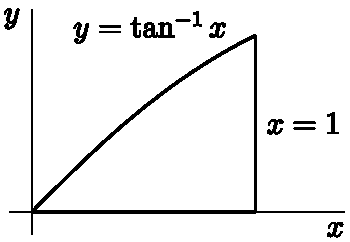
\includegraphics{graphE4bl}
\end{center}
\noindent (b) Volume: $ \dfrac{\pi^2}{2}-\pi$
\end{answer}

\begin{solution} (a) The sketch is the figure on  the left below.
By integration by parts with $u=\arctan x$, $\dee{v}=\dee{x}$,  $v=x$ and $\dee{u}=\frac{1}{1+x^2}\,\dee{x}$, and then the substitution $s=1+x^2$,
\begin{align*}
A&=\int_0^1\arctan x\ \dee{x}=\underbrace{ x\arctan x}_{uv}\Big|_0^1-\int_0^1\underbrace{\frac{x}{1+x^2}\,\dee{x}}_{v\dee{u}}
=\arctan 1-\half\log(1+x^2)\Big|_0^1\\
&=\frac{\pi}{4}-\frac{\log 2}{2}
\end{align*}

\begin{center}
       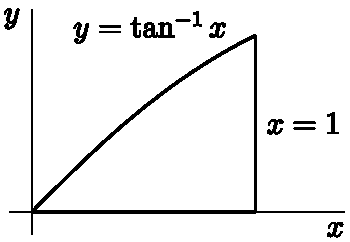
\includegraphics{graphE4bl}\qquad
       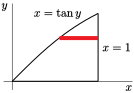
\includegraphics{graphE4br}
\end{center}

\noindent (b)
We'll use horizontal washers as in Example  \eref{CLP101}{eg rot yaxis}
of the %\href{http://www.math.ubc.ca/%7Efeldman/m101/clp/clp_notes_101.pdf}{CLP 101 notes}.
CLP--II text.
 \begin{itemize}
\item We cut $R$ into thin horizontal  strips of width $\dee{y}$ as in
the figure on the right above.

\item When we rotate $R$ about the $y$--axis, each strip sweeps out a thin
washer
\begin{itemize}
\item whose inner radius is $r_{in}=\tan y$ and outer radius is $r_{out}=1$, and
\item whose thickness is $\dee{y}$ and hence
\item whose volume $\pi(r_{out}^2 - r_{in}^2)\dee{y} = \pi(1-\tan^2 y)\dee{y}$.
\end{itemize}
\item As our bottommost strip is at $y=0$ and our topmost
strip is at $y=\frac{\pi}{4}$ (since at the top $x=1$ and $x=\tan y$), the total
\begin{align*}
\text{Volume}
&= \int _0^{\nicefrac{\pi}{4}} \pi(1-\tan^2 y)\ \dee{y}
= \int _0^{\nicefrac{\pi}{4}} \pi(2-\sec^2 y)\ \dee{y}
=\pi\big[2y -\tan y\big]_0^{\nicefrac{\pi}{4}} \\
&= \frac{\pi^2}{2}-\pi
\end{align*}
\end{itemize}
\end{solution}

%%%%%%%%%%%%%%%%%%%
%%%%%%%%%%%%%%%%%%%

\begin{question}[2016Q3] %% 6
Let $R$ be the region between the curves $T(x) = \sqrt{x}e^{3x}$ and $B(x) = \sqrt{x}(1+2x)$ on the interval $0 \le x \le 3$. (It is true that $T(x)\ge B(x)$ for all $0\le x\le 3$.) Compute the volume of the solid formed by rotating $R$ about the $x$-axis.
\end{question}

\begin{hint}
Your integral can be broken into two integrals, which yield to two different integration methods.
\end{hint}

\begin{answer}
$ \pi \left( \dfrac{17 e^{18}-4373}{36} \right)$
\end{answer}

\begin{solution}
For a fixed value of $x$, if we rotate about the $x$-axis, we form a washer of
inner radius $B(x)$ and outer radius $T(x)$ and hence of area $\pi [T(x)^2 - B(x)^2]$.
We integrate this function from $x=0$ to $x=3$ to find the total volume~$V$:
\begin{align*}
V &= \int_0^3 \pi [T(x)^2 - B(x)^2]\,\dee{x} \\
&= \pi \int_0^3 (\sqrt{x}e^{3x})^2 - (\sqrt{x}(1+2x))^2 \,\dee{x} \\
&= \pi \int_0^3  \big( xe^{6x} - (x+4x^2+4x^3) \big) \,\dee{x} \\
&=  \pi \int_0^3 xe^{6x} \,\dee{x}
       - \pi  \Big[ \frac{x^2}{2} + \frac{4x^3}{3} + x^4\Big]_{0}^3 \\
&= \pi \int_0^3 xe^{6x} \,\dee{x} - \pi \Big[\frac{3^2}{2} + \frac{4\cdot3^3}{3} + 3^4\Big]
\end{align*}
For the first integral, we use integration by parts with $u(x) = x$, $\dee{v} = e^{6x}\dee{x}$,
so that $\dee{u}=\dee{x}$ and $v(x)=\frac16e^{6x}$:
\begin{align*}
\int_0^3 xe^{6x} \,\dee{x}
&=\underbrace{ \frac{xe^{6x}}{6}}_{uv}\bigg|_{0}^3 - \int_0^3 \underbrace{\frac{1}{6}e^{6x} \,\dee{x} }_{v\dee{u}}\\
&= \frac{3e^{18}}{6} - 0 - \frac{1}{36} e^{6x} \bigg|_{0}^3
= \frac{e^{18}}{2} - \bigg( \frac{e^{18}}{36} - \frac1{36} \bigg).
\end{align*}
Therefore, the total volume is
\begin{align*}
  V = \pi \bigg[\frac{e^{18}}{2} - \bigg( \frac{e^{18}}{36} - \frac1{36} \bigg) \bigg]
               - \pi \bigg[\frac{3^2}{2} + \frac{4\cdot3^3}{3} + 3^4 \bigg]
    = \pi \bigg( \frac{17 e^{18}-4373}{36} \bigg).
\end{align*}
\end{solution}
%%%%%%%%%%%%%%%%%%%

\begin{Mquestion}[M105 2013A]
Let $f(0) = 1$, $f(2) = 3$ and $f'(2) = 4$.
Calculate
${\displaystyle\int_0^4 f''\big(\sqrt{x}\big)\,\dee{x}}$.
\end{Mquestion}

\begin{hint}
Think, first, about how to get rid of the square root in the argument of $f''$,
and, second, how to convert $f''$ into $f'$. Note that you are told that $f'(2) = 4$
and $f(0) = 1$, $f(2) = 3$.
\end{hint}

\begin{answer}
$12$
\end{answer}

\begin{solution}
To get rid of the square root in the argument of $f''$, we make the change of variables (also called ``substitution")
$x=t^2,\ \dee{x}=2t\,\dee{t}$.
\begin{align*}
\int_0^4 f''\big(\sqrt{x}\big)\,\dee{x}
&= 2\int_0^2 tf''(t)\,\dee{t}
\end{align*}
Then, to convert $f''$ into $f'$, we  integrate by parts with
$u=t$,  $\dee{v}=f''(t)\,\dee{t}$,    $v=f'(t) $.
\begin{align*}
\int_0^4 f''\big(\sqrt{x}\big)\,\dee{x}
&= 2\bigg\{\Big[\underbrace{tf'(t)}_{uv}\Big]_0^2-\int_0^2\!\!\!\underbrace{ f'(t)\,\dee{t}}_{v\dee{u}}\bigg\} \\
&=2\Big[tf'(t)-f(t)\Big]_0^2 \\
&=2\big[2f'(2)-f(2)+f(0)\big]=2\big[2\times 4-3+1\big]\\
&=12
\end{align*}


\end{solution}

%%%%%%%%%%%%%%%%%%%
\begin{question}
Evaluate $\displaystyle\lim_{n \to \infty}\sum_{i=1}^n \frac{2}{n}\left(\frac{2}{n}i-1\right)e^{\frac{2}{n}i-1}$\ .
\end{question}
\begin{hint}
Interpret the limit as a right Riemann sum.
\end{hint}
\begin{answer}
$\dfrac{2}{e}$
\end{answer}
\begin{solution}
As we saw in Section~\eref{CLP101}{sec:intdef} of the CLP--II text, there are many different ways to interpret a limit as a Riemann sum. In the absence of instructions that restrain our choices, we go with the most convenient interpretations.

With that in mind, we choose:
\begin{itemize}
\item that our Riemann sum is a right Riemann sum (because we see $i$, not $i-1$ or $i-\frac{1}{2}$)
\item $\Delta x = \frac{2}{n}$ (because it is multiplied by the rest of the integrand, and also shows up multiplied by $i$),
\item then $x_i = a+i\Delta x = \frac{2}{n}i-1$, which leads us to $a=-1$ and
\item $f(x) = xe^x$.
\item Finally, since $\Delta x = \frac{b-a}{n}=\frac{2}{n}$ and $a=-1$, we have $b=1$.
\end{itemize}

So, the limit is equal to the definite integral
\begin{align*}
\lim_{n \to \infty}\sum_{i=1}^n \frac{2}{n}\left(\frac{2}{n}i-1\right)e^{\frac{2}{n}i-1}&=\int_{-1}^1x e^x~\dee{x}
\intertext{which we evaluate using integration by parts with $u=x$, $\dee{v}=e^x\dee{x}$, $\dee{u}=\dee{x}$, and $v=e^x$.}
&=\Big[\underbrace{xe^x}_{uv} \Big]_{-1}^1 - \int_{-1}^1 \underbrace{e^x\dee{x}}_{v\dee{u}}\\
&=\left(e+\frac{1}{e}\right) - \left(e-\frac{1}{e}\right) = \frac{2}{e}
\end{align*}
\end{solution}
